\documentclass[12pt]{article}

\newcommand{\name}{Jonathan Homburg}

\usepackage{algorithm2e}
\usepackage{amsfonts}
\usepackage{amssymb}
\usepackage{amsmath}
\usepackage{amsthm}
\usepackage{mathtools}
\usepackage{centernot}
\usepackage{changepage}
\usepackage{framed}
\usepackage{graphicx}
\usepackage{latexsym}
\usepackage{enumerate}
\usepackage{tikz}
\usepackage{pgfplots}
\usepackage{verbatim}

\usepackage[final]{hyperref} % adds hyper links inside the generated pdf file
\hypersetup{
	colorlinks=true,       % false: boxed links; true: colored links
	linkcolor=blue,          % color of internal links
	citecolor=blue,        % color of links to bibliography
	filecolor=magenta,      % color of file links
	urlcolor=blue         %%% from template
}

\setlength{\parskip}{1pc}
\setlength{\parindent}{0pt}
\setlength{\topmargin}{-3pc}
\setlength{\textheight}{9.5in}
\setlength{\oddsidemargin}{0pc}
\setlength{\evensidemargin}{0pc}
\setlength{\textwidth}{6.5in}

\long\def\/*#1*/{}

\newtheorem{theorem}{Theorem}
\newtheorem{mydef}{Definition}
\newtheorem{lemma}[theorem]{Lemma}
\newtheorem{remark}{Remark}

\DeclarePairedDelimiter\abs{\lvert}{\rvert}
\DeclarePairedDelimiter{\ceil}{\lceil}{\rceil}
\DeclarePairedDelimiter{\floor}{\lfloor}{\rfloor}

\makeatletter
\let\oldabs\abs
\def\abs{\@ifstar{\oldabs}{\oldabs*}}

\let \classicphi \phi
\def \phi{\varphi}
\let \classicepsilon \epsilon
\def \epsilon{\varepsilon}

\newcommand{\suchthat}{\hphantom l | \hphantom l}
\newcommand{\normaleq}{\trianglelefteq}
\newcommand{\ZZ}{\mathbb{Z}}
\newcommand{\RR}{\mathbb{R}}
\newcommand{\QQ}{\mathbb{Q}}
\newcommand{\CC}{\mathbb{C}}

\DeclareMathOperator{\Tor}{Tor}
\DeclareMathOperator{\Aut}{Aut}
\DeclareMathOperator{\Inn}{Inn}
\DeclareMathOperator{\Syl}{Syl}

\usetikzlibrary{arrows}

\begin{document}
This document consists of a breakdown of the current state and design plan of our project, as I understand it. My goal was to organize a lot of the design notes and decisions spread out across most of our meetings into a single document and then combine that with a description of the current state of our project. It is still pretty rough though and could probably use some revision. Let me know if I forgot or misunderstood anything.

A diagram of the overview for the structure of our project is given below:
\begin{center}
\begin{tikzpicture}[trans/.style={thick,->,shorten >=2pt,shorten <=2pt,>=stealth}]
\node[draw,rectangle,align=center](A)  at (1,0)
	{\textbf{Input:} \\ markdown with \\ code blocks for \\ 	 visualization};
\node[draw,rectangle,align=center](B)  at (1,-2.5) 
	{\textbf{Task 1}: \\ identify blocks \\ of code};
\node[draw,rectangle,align=center](C)  at (1,-5.5) 
	{\textbf{Task 2}: \\ process code blocks \\ into recognized \\ data structures \\ and algorithms};
\node[draw, rectangle, align=center](D) at (1,-8.5)
	{\textbf{Task 3}: \\ Create SVG \\ visualizations};
\node[draw, rectangle, align=center](E) at (1,-11)
	{\textbf{Task 4}: \\ Replace tool-specific \\ language in input \\ with SVG visualizations};
\node[draw, rectangle, align=center](F) at (1,-13.5)
	{\textbf{Output}: \\ Makrdown file \\ with visualizations};
\draw[trans] (A) -- (B);
\draw[trans] (B) -- (C);
\draw[trans] (C) -- (D);
\draw[trans] (D) -- (E);
\draw[trans] (E) -- (F);
\end{tikzpicture}
\end{center}

I don't plan to describe in detail why we decided to use the modular structure described above, see Oliver's components.md for that. Currently, Anna, John, Doni and I are working on task 3 (visualization) while Oliver and Eyal are working on task 2 (description).

Detailed descriptions of the above tasks are given below. I also include (my understanding of) the current state of our progress on these tasks. 

\subsection*{Tool 1: Identifying code blocks}

Our project will be given a markdown file with user-defined blocks of code and descriptions of how/what they want visualized.The task of this component will be to identify these subsections of the input markdown and then pass these on to the second tool. Doni has started work on this.

\subsection*{Tool 2: Describing data structures}
After the first tool identifies the relevant code and description of how it will be visualized, it is the task of this tool to create a language-independent description of the data structure and pass it on to the next tool for visualization. 

The first task of this tool is processing the given code block to understand what it is trying to represent. Our current plan for this is to have a user implement an "identifier" class for each data structure that they want visualized. This identifier will implement all of the functions that our tools needs access to in order to understand the structure and contents of the data structure. The motivation for this is that a user may want to visualize the same instance of a class in different ways (e.g. visualizing a tree as a tree proper and later as a generic graph) and this allows us to never need to interact with the user's actual code (ideally). 

For an example of the above, see Oliver's tree\_visitor\_example.py. In this file, we have the following classes:
\begin{enumerate}
\item BinaryTreeIdentifier (Visualizer-defined Abstract Identifier): An abstract class that defines what functions we need the user to implement to properly visualize the tree
\item BinaryTreeVisitor (Visualizer-defined Vistitor): The internal function in our code that uses the user-defined implementation of BinaryTreeIdentifier to traverse the given tree and extract the information needed for visualization.
\item UselessBinaryTree (User-defined Internal Class): The tree class that the user defines to use locally. Our code will ideally never touch this class.
\item UselessBinaryTreeIdentifier (User-defined Identifier): Implements the abstract BinaryTreeIdentifier class. The user defines how to gather the relevant information from UselessBinaryTree.
\end{enumerate}

A general diagram of the relationships between these classes is given below:

\begin{center}
\begin{tikzpicture}[trans/.style={thick,->,shorten >=2pt,shorten <=2pt,>=stealth}]
\node[draw,rectangle,align=center, minimum height = 4cm, minimum width =3cm, text height = -3cm]  at (1,0)
	{\textbf{Visualizer}};
	\node[draw,rectangle,align=center](A)  at (1,0.5){Abstract \\ Identifier};
	\node[draw,rectangle,align=center](B)  at (1,-1){Visitor};
\node[draw,rectangle,align=center, minimum height = 4cm, minimum width =3cm, text height = -3cm]  at (5,0)
	{\textbf{User Code}};
	\node[draw,rectangle,align=center](C)  at (5,0.5){Identifier};
	\node[draw,rectangle,align=center](D)  at (5,-1){Internal \\ Classes};
	\draw[trans] (B) -- (A);
	\draw[trans] (A) -- (C);
	\draw[trans] (C) -- (D);
\end{tikzpicture}
\end{center}

Although we have a working instance of the above specifically for trees, we do not yet have any other data structure implemented.

After the relevant information is parsed from the user's code, this tool also has the task of writing a language-independent description of the contents so that we visualize it with the next tool. Oliver has taken to calling these description "UConn Language Independent Descriptions of Structures" or UCLIDS. Oliver and Eyal have begun working on a formal specification of the UCLIDS format. The work that has been done on this so far is in UCLIDS\_spec.md.

\subsection*{Tool 3: Visualzing Data Structures}
All relevant information about the structure and contents of a data structure should be contained in the UCLIDS description and then passed to the visualizer. Thus, the visualizer only needs to concern itself with how to best visualize (i.e. generate an SVG representing) a given data structure (it need not worry about parsing/processing other code). This is not so simple of a task though.

To start, we've identified a few crucial (and relatively simple) data structures and are implementing these independently. These starting data structures are trees, linked lists, sets, and arrays. This is what we are working on now. Once that is finished, we will merge our ideas into a common visualization framework and design. After this, it will be pretty straight forward to add a new data structure for visualization (at least for this tool) assuming that we can figure out how to visualize them.

So far, I've implemented a visualizer for trees and John has implemented a visualizer for linked lists. I believe Anna is working on sets and Doni is working on arrays. The code that we have finished can be viewed at https://github.com/Agizin/Algorithm-Visualization.

\subsection*{Tool 4: Adding SVG to Markdown}
This tool needs to remove the code in the markdown file specific to our visualizer (i.e. probably the identifier code described under Tool 2) and add the SVGs file given as output by the previous component. This is the tool that we've worked least on but I also suspect that it will not give us much trouble. 
\end{document}